%! TeX program = lualatex
\documentclass[12pt]{article}

\usepackage{cmap}
\usepackage{newfloat}
\usepackage[newfloat]{minted}
\usepackage[font=small]{caption}
\usepackage{indentfirst}

\setminted{
    linenos,                % показывать номера строк
    breaklines,             % переносить длинные строки
    breakanywhere=true,     % переносить в любом месте
    tabsize=2,              % размер табуляции
    fontsize=\scriptsize,        % размер шрифта
    frame=lines,            % рамка сверху и снизу
    framesep=2mm,           % расстояние текста от рамки
    baselinestretch=1.1,    % межстрочный интервал
    autogobble=true,        % автоудаление общего отступа
    % xleftmargin=10pt,       % отступ слева
    % numbersep=5pt,          % расстояние между номерами и кодом
}

\usepackage[english, russian]{babel}

\usepackage[nopatch=footnote]{microtype}

\usepackage{float}
\usepackage{fontspec}
\usepackage[pdfborder={0 0 0}]{hyperref}

\usepackage{enumitem}

\makeatletter
\renewcommand\@seccntformat[1]{%
  \csname the#1\endcsname.\quad
}
\makeatother

\usepackage{tocloft}
\renewcommand{\cftsecaftersnum}{.}
\renewcommand{\cftsubsecaftersnum}{.}
\renewcommand{\cftsubsubsecaftersnum}{.}

\setmainfont{TimesNewerRoman}[
  Extension = .otf,
  Path = /nix/store/ihdqrn4p54awd89vrday9k53s8i47bbv-times-newer-roman-unstable-2018-09-11/share/fonts/opentype/,
  UprightFont = *-Regular,
  BoldFont = *-Bold
]
\setmonofont{Ubuntu Mono}

\newcommand{\icon}[1]{\fontspec{UbuntuNerdFont}[Extension = .ttf,
  Path = /nix/store/h721jafy2n74x4k5p0hxbz722h0rncmx-nerd-fonts-ubuntu-3.3.0+0.83/share/fonts/truetype/NerdFonts/Ubuntu/,
  UprightFont = *-Regular,
BoldFont = *-Bold] #1}

\newcommand{\iicon}[1]{{\icon{#1}}}

\usepackage{graphicx}
\usepackage{fontawesome5} % Для иконок

\usepackage[left=2.0cm, right=2.0cm, top=1.0cm, bottom=1.0cm, includeheadfoot]{geometry}

% \usepackage[mocha, textcolor=true, pagecolor=true]{catppuccinpalette} \usemintedstyle{catppuccin-mocha}
\usepackage[latte, textcolor=true, pagecolor=true]{catppuccinpalette} \usemintedstyle{catppuccin-latte}

\usepackage{setspace}
\onehalfspacing

\usepackage{fancyhdr}
\fancyhf{}

\renewcommand{\sectionmark}[1]{\markboth{#1}{}}
\renewcommand{\subsectionmark}[1]{\markright{#1}}

% Настройка колонтитулов
\fancyhead[RO]{\rightmark}
\fancyhead[LO]{\leftmark}

\fancyfoot[L]{\hspace{8pt} \rule{\textwidth}{0.4pt}}
\fancyfoot[R]{\LARGE{\thepage}}
\fancyfoot[C]{}

\newcommand{\lablogo}
{
\begin{center}
    \huge{\textbf{Лабораторная работа №4}} \\
\end{center}
}

\newcommand{\colorURL}[1]{\textcolor{CtpBlue}{#1}}
\newcommand{\colorGIT}[1]{\textcolor{CtpLavender}{#1}}
\renewcommand{\texttt}[1]{{\small\ttfamily #1}}

\setlength{\headheight}{15.2pt}

\DeclareCaptionLabelFormat{gostfigure}{Рисунок #2}
\captionsetup[figure]{labelformat=gostfigure, labelsep=endash}

\DeclareCaptionLabelFormat{gostlisting}{Листинг #2}
\newenvironment{code}{\captionsetup{type=listing}}{}
\captionsetup[listing]{labelformat=gostlisting, labelsep=endash}
\DeclareFloatingEnvironment[
  listname=Листинг,
]{listing}

\usepackage{amsmath}
\numberwithin{listing}{section}
\numberwithin{figure}{section}

\usepackage{tocloft}
\renewcommand{\cftsecleader}{\cftdotfill{\cftdotsep}}

\begin{document}
\pagestyle{empty}
\lablogo
\tableofcontents
\listoflistings
\newpage

\pagestyle{fancy}

\section{Цель работы~\texorpdfstring{\iicon{}}{}}
Освоить принципы построения приложений на WPF с применением паттерна MVVM, базы данных SQLite и технологии Entity Framework Core. Разработать функциональность управления товарами и заказами в рамках настольного приложения.

\noindent \textbf{Задание:}
\begin{enumerate}
	\item Изучить архитектуру MVVM и реализовать её на практике.
	\item Использовать Entity Framework Core для доступа к базе данных.
	\item Организовать взаимодействие между слоями модели, представления и логики представления.
	\item Настроить графический интерфейс пользователя для работы с товарами и заказами.
	\item Реализовать команды добавления, редактирования и удаления данных.
\end{enumerate}

\pagebreak

\section{Теоретические сведения~\texorpdfstring{\iicon{}}{}}
StoreManager — это настольное WPF-приложение на платформе .NET, реализующее базовую функциональность управления магазином: добавление/редактирование товаров, формирование заказов, управление корзиной, отображение и удаление заказов. Проект построен по принципам MVVM (Model-View-ViewModel), использует Entity Framework Core для работы с SQLite базой данных.

\noindent \textbf{Основные компоненты:}
\begin{itemize}
	\item Model: классы \texttt{Product}, \texttt{Order}, \texttt{OrderItem}, \texttt{CartItem} — описывают бизнес-логику и данные.
	\item ViewModel: классы \texttt{MainViewModel}, \texttt{ProductViewModel}, \texttt{OrderViewModel} управляют состоянием и взаимодействием между представлением и моделью.
	\item View: XAML-интерфейс, представляющий UI, привязанный к ViewModel.
\end{itemize}

\noindent \textbf{Используемые технологии:}
\begin{itemize}
	\item C\#, .NET
	\item WPF (XAML)
	\item Entity Framework Core
	\item SQLite
	\item MVVM-паттерн
\end{itemize}

\pagebreak

\section{Порядок выполнения работы~\texorpdfstring{\iicon{󰈍}}{}}
В данном разделе последовательно описан процесс подготовки, запуска и анализа исходного кода проекта. Необходимо \textcolor{CtpRed}{строго} придерживаться шагов, описанных ниже, чтобы успешно воспроизвести и исследовать функциональность приложения.

\begin{enumerate}
	\item Для начала необходимо открыть проект в среде разработки Visual Studio.
	\item Далее необходимо установить требуемые библиотеки через NuGet Package Manager. Список необходимых NuGet-пакетов:
	      \begin{itemize}
		      \item \texttt{Microsoft.EntityFrameworkCore}
		      \item \texttt{Microsoft.EntityFrameworkCore.Sqlite}
		      \item \texttt{Microsoft.Data.Sqlite}
	      \end{itemize}
\end{enumerate}

\subsection{Первичная настройка базы данных}
После установки зависимостей необходимо выполнить инициализацию базы данных. При первом запуске приложение автоматически создаёт файл базы данных \texttt{store.db} с помощью метода \texttt{EnsureCreated()}.

\subsection{Запуск проекта}
После выполнения всех предыдущих шагов необходимо запустить приложение. Проект \texttt{Store\-Manager\_4lab} должен быть выбран в качестве стартового.

\pagebreak

\noindent \section{Исходный код и комментарии~\texorpdfstring{\iicon{}}{}}
В данном разделе рассмотрены ключевые компоненты проекта, реализующие бизнес-логику и связь с пользовательским интерфейсом. Далее последовательно представлены листинги кода с пояснениями.

\subsection{\texttt{RelayCommand.cs} — реализация команды MVVM}
\begin{code}
	\begin{minted}[linenos, fontsize=\footnotesize, frame=lines]{csharp}
public class RelayCommand : ICommand
{
    private readonly Action<object> _execute; // делегат выполнения команды
    private readonly Func<object, bool> _canExecute; // делегат проверки возможности выполнения команды

    // Конструктор команды
    public RelayCommand(Action<object> execute, Func<object, bool> canExecute = null)
    {
        _execute = execute ?? throw new ArgumentNullException(nameof(execute)); // инициализация метода выполнения
        _canExecute = canExecute; // инициализация метода проверки доступности
    }

    // Событие, которое вызывается при изменении условий выполнения команды
    public event EventHandler CanExecuteChanged
    {
        add { CommandManager.RequerySuggested += value; }
        remove { CommandManager.RequerySuggested -= value; }
    }

    // Проверка, может ли команда быть выполнена
    public bool CanExecute(object parameter) => _canExecute?.Invoke(parameter) ?? true;

    // Выполнение команды
    public void Execute(object parameter) => _execute(parameter);
}
    \end{minted}
	\captionof{listing}{Класс RelayCommand}
	\label{lst:RelayCommand}
\end{code}
В листинге \ref{lst:RelayCommand} представлен класс \texttt{RelayCommand}. Данный класс реализует интерфейс \texttt{ICommand}, что позволяет привязывать действия в UI к методам ViewModel. Применяется для реализации кнопок и команд.

\begin{enumerate}
	\item \texttt{RelayCommand(...)} — конструктор команды. Принимает делегаты выполнения и условия выполнения. Используется при создании команд в ViewModel.
	\item \texttt{CanExecute(object parameter)} — возвращает true, если команду можно выполнить. Применяется для активации/деактивации элементов интерфейса.
	\item \texttt{Execute(object parameter)} — запускает делегат действия команды. Вызывается при клике на кнопку или другое действие пользователя.
\end{enumerate}

\subsection{\texttt{StoreDbContext.cs} — контекст базы данных}
\begin{code}
	\begin{minted}[linenos, fontsize=\footnotesize, frame=lines]{csharp}
public class StoreDbContext : DbContext
{
    // Таблица товаров
    public DbSet<Product> Products { get; set; }
    // Таблица заказов
    public DbSet<Order> Orders { get; set; }
    // Таблица позиций заказа
    public DbSet<OrderItem> OrderItems { get; set; }
    // Конфигурация подключения к базе данных
    protected override void OnConfiguring(DbContextOptionsBuilder optionsBuilder)
    {
        optionsBuilder.UseSqlite("Data Source=store.db"); // указание строки подключения к SQLite
    }
    // Настройка модели данных
    protected override void OnModelCreating(ModelBuilder modelBuilder)
    {
        modelBuilder.Entity<Order>()
            .HasMany(o => o.Items) // один заказ содержит множество позиций
            .WithOne()             // без явной обратной связи
            .OnDelete(DeleteBehavior.Cascade); // при удалении заказа удаляются все его позиции
    }
}
    \end{minted}
	\captionof{listing}{Контекст базы данных}
	\label{lst:StoreDbContext}
\end{code}

\begin{enumerate}
	\item \texttt{OnConfiguring(DbContextOptionsBuilder optionsBuilder)} — вызывается при создании экземпляра контекста. Устанавливает строку подключения к базе данных SQLite.
	\item \texttt{OnModelCreating(ModelBuilder modelBuilder)} — выполняется при инициализации модели EF. Здесь настраивается каскадное удаление зависимых сущностей (например, позиций заказа при удалении заказа). Определяет три таблицы: \texttt{Product}, \texttt{Order}, \texttt{OrderItem}.
\end{enumerate}

\subsection{\texttt{CartItem.cs} — элемент корзины}
Далее представлен листинг класса \texttt{CartItem}, отвечающего за временное хранение товаров (Листинг \ref{lst:CartItem}).
\begin{code}
	\begin{minted}[linenos, fontsize=\footnotesize, frame=lines]{csharp}
public class CartItem : INotifyPropertyChanged
{
    public Product Product { get; set; } // ссылка на продукт

    private int _quantity; // поле для хранения количества

    public int Quantity
    {
        get => _quantity; // получение значения
        set { _quantity = value; OnPropertyChanged(); } // установка значения и уведомление об изменении
    }

    // Событие, уведомляющее об изменении свойства
    public event PropertyChangedEventHandler PropertyChanged;

    // Метод вызова события изменения свойства
    protected void OnPropertyChanged([CallerMemberName] string name = null) =>
        PropertyChanged?.Invoke(this, new PropertyChangedEventArgs(name));
}
    \end{minted}
	\captionof{listing}{Листинг «Корзины товаров»}
	\label{lst:CartItem}
\end{code}
\texttt{CartItem} служит для временного хранения товаров в корзине перед созданием заказа. Используется в \texttt{ObservableCollection<CartItem>}.

\begin{enumerate}
	\item \texttt{Product} — ссылка на экземпляр товара, связанный с объектом корзины.
	\item \texttt{Quantity} — количество выбранного товара в корзине. При изменении уведомляет UI через механизм \texttt{INotifyPropertyChanged}.
	\item \texttt{OnPropertyChanged(string name)} — метод, вызывающий событие \texttt{PropertyChanged} для обновления интерфейса при изменении свойств.
\end{enumerate}

\subsection{\texttt{MainViewModel.cs} — основная логика взаимодействия с UI}
\begin{code}
	\begin{minted}[linenos, fontsize=\footnotesize, frame=lines]{csharp}
public class MainViewModel : INotifyPropertyChanged
{
    // Контекст базы данных
    private readonly StoreDbContext _context = new();

    // Коллекция всех товаров
    public ObservableCollection<Product> Products { get; set; } = new();

    // Коллекция всех заказов
    public ObservableCollection<Order> Orders { get; set; } = new();

    // Коллекция товаров, добавленных в корзину
    public ObservableCollection<CartItem> CartItems { get; } = new();

    // Команда добавления товара
    public ICommand AddProductCommand { get; }

    // Команда создания заказа
    public ICommand AddOrderCommand { get; }

    // Конструктор ViewModel
    public MainViewModel()
    {
        // Инициализация команд
        AddProductCommand = new RelayCommand(_ => AddProduct(), _ => CanAddProduct());
        AddOrderCommand = new RelayCommand(_ => AddOrder());

        // Создание базы данных при первом запуске
        _context.Database.EnsureCreated();

        // Загрузка данных из базы
        LoadProducts();
        LoadOrders();
    }

    // Загрузка всех товаров из базы данных
    private void LoadProducts()
    {
        Products.Clear();
        foreach (var p in _context.Products.ToList())
            Products.Add(p);
    }

    // Загрузка всех заказов с товарами из базы данных
    private void LoadOrders()
    {
        Orders.Clear();
        var allOrders = _context.Orders
            .Include(o => o.Items)
            .ThenInclude(i => i.Product)
            .ToList();

        foreach (var order in allOrders)
            Orders.Add(order);
    }

    // Добавление нового товара
    private void AddProduct()
    {
        var product = new Product
        {
            Name = "Новый товар",     // название товара
            Price = 100,              // цена по умолчанию
            Stock = 10,               // количество по умолчанию
            Category = "Общая"        // категория товара
        };

        _context.Products.Add(product);     // добавление в базу данных
        _context.SaveChanges();             // сохранение изменений
        LoadProducts();                     // обновление списка товаров
    }

    // Добавление нового заказа
    private void AddOrder()
    {
        if (!CartItems.Any()) return; // проверка наличия товаров в корзине

        var order = new Order
        {
            CustomerName = "Клиент", // имя покупателя
            OrderDate = DateTime.Now, // дата оформления
            Items = CartItems.Select(c => new OrderItem
            {
                Product = c.Product,    // товар
                Quantity = c.Quantity   // количество
            }).ToList()
        };

        _context.Orders.Add(order);   // добавление заказа в БД
        _context.SaveChanges();       // сохранение
        LoadOrders();                 // обновление списка
        CartItems.Clear();            // очистка корзины
    }

    // Условие доступности команды добавления товара
    private bool CanAddProduct() => true;

    public event PropertyChangedEventHandler PropertyChanged;

    // Обработка события изменения свойства
    protected void OnPropertyChanged([CallerMemberName] string name = null) =>
        PropertyChanged?.Invoke(this, new PropertyChangedEventArgs(name));
}
    \end{minted}
	\captionof{listing}{Логика взаимодействия с UI}
	\label{lst:MainViewModel}
\end{code}
В листинге \ref{lst:MainViewModel} представлен код класса \texttt{MainViewModel}. Он связывает данные с пользовательским интерфейсом. В нём реализованы команды для добавления товаров и заказов, загрузка данных из базы и взаимодействие с коллекциями. Этот класс является ядром логики MVVM и предоставляет интерфейс между XAML и данными модели.


\begin{enumerate}
	\item \texttt{MainViewModel()} — конструктор класса. Производит инициализацию базы, загрузку данных и настройку команд.
	\item \texttt{LoadProducts()} — загружает все товары из базы данных в \texttt{ObservableCollection} для отображения.
	\item \texttt{LoadOrders()} — загружает все заказы и их связанные товары.
	\item \texttt{AddProduct()} — добавляет новый товар в базу и обновляет отображаемый список.
	\item \texttt{AddOrder()} — формирует и сохраняет заказ на основе содержимого корзины.
	\item \texttt{CanAddProduct()} — всегда возвращает true, используется как условие для активности команды добавления товара.
	\item \texttt{OnPropertyChanged(string name)} — реализует уведомление об изменении свойства, используется в привязках.
\end{enumerate}

\subsection{Репозиторий \texttt{ProductRepository.cs} — операции с товарами}
\begin{code}
	\begin{minted}[linenos, fontsize=\footnotesize, frame=lines]{csharp}
public class ProductRepository
{
    private const string ConnectionString = "Data Source=store.db"; // строка подключения к базе данных

    public List<Product> GetAll()
    {
        var list = new List<Product>(); // список для хранения всех продуктов
        using var connection = new SqliteConnection(ConnectionString); // открытие соединения с базой данных
        connection.Open(); // выполнение подключения к базе данных

        var command = connection.CreateCommand(); // создание SQL-команды
        command.CommandText = "SELECT * FROM Product"; // выборка всех записей из таблицы товаров

        using var reader = command.ExecuteReader(); // выполнение команды и получение результатов
        while (reader.Read()) // построчное чтение результатов
        {
            list.Add(new Product // добавление экземпляра товара в список
            {
                Id = reader.GetInt32(0), // идентификатор товара
                Name = reader.GetString(1), // название товара
                Price = reader.GetDecimal(2), // цена товара
                Stock = reader.GetInt32(3), // остаток товара на складе
                Category = reader.IsDBNull(4) ? null : reader.GetString(4) // категория товара (может отсутствовать)
            });
        }
        return list; // возвращение списка всех товаров
    }

    public void Add(Product product)
    {
        using var connection = new SqliteConnection(ConnectionString); // открытие соединения с базой данных
        connection.Open(); // выполнение подключения к БД

        var command = connection.CreateCommand(); // создание SQL-команды
        command.CommandText = "INSERT INTO Product (Name, Price, Stock, Category) VALUES (@name, @price, @stock, @category)"; // вставка нового товара в таблицу Product
        command.Parameters.AddWithValue("@name", product.Name); // название товара
        command.Parameters.AddWithValue("@price", product.Price); // цена товара
        command.Parameters.AddWithValue("@stock", product.Stock); // количество товара на складе
        command.Parameters.AddWithValue("@category", product.Category ?? (object)DBNull.Value); // категория товара (или null)

        command.ExecuteNonQuery(); // выполнение SQL-команды
    }
}
    \end{minted}
	\captionof{listing}{Основные операции с товарами}
	\label{lst:ProductRepository}
\end{code}
Класс \texttt{ProductRepository} предоставляет низкоуровневый доступ к таблице товаров. В нём реализованы методы чтения и добавления продуктов с использованием SQLite.


\begin{enumerate}
	\item \texttt{GetAll()} — выполняет подключение к базе данных и извлекает все товары из таблицы \texttt{Product}. Используется при загрузке списка товаров в интерфейсе.
	\item \texttt{Add(Product product)} — добавляет новый товар в базу данных с помощью SQL-запроса \texttt{INSERT}. Используется при создании новых товаров пользователем.
\end{enumerate}

\subsection{Репозиторий \texttt{OrderRepository.cs} — работа с заказами}
\begin{code}
	\begin{minted}[linenos, fontsize=\footnotesize, frame=lines]{csharp}
public class OrderRepository
{
    private const string ConnectionString = "Data Source=store.db"; // строка подключения к БД

    public List<Order> GetAll(List<Product> allProducts)
    {
        var orders = new List<Order>(); // список заказов
        using var connection = new SqliteConnection(ConnectionString); // открытие соединения с базой данных
        connection.Open(); // выполнение подключения

        var command = connection.CreateCommand(); // создание SQL-команды
        command.CommandText = "SELECT Id, CustomerName, OrderDate FROM [Order]"; // выборка данных заказов
        using var reader = command.ExecuteReader(); // выполнение запроса и чтение результатов

        while (reader.Read()) // построчное чтение результата
        {
            var order = new Order
            {
                Id = reader.GetInt32(0), // идентификатор заказа
                CustomerName = reader.GetString(1), // имя клиента
                OrderDate = DateTime.Parse(reader.GetString(2)), // дата оформления заказа
                Items = new List<OrderItem>() // список товаров в заказе
            };
            orders.Add(order); // добавление заказа в коллекцию
        }

        foreach (var order in orders) // обход заказов для загрузки позиций
        {
            var itemCmd = connection.CreateCommand(); // создание SQL-команды для выбора позиций заказа
            itemCmd.CommandText = "SELECT ProductId, Quantity FROM OrderItem WHERE OrderId = @orderId"; // выборка товарных позиций
            itemCmd.Parameters.AddWithValue("@orderId", order.Id); // параметр: идентификатор заказа
            using var itemReader = itemCmd.ExecuteReader(); // выполнение запроса

            while (itemReader.Read()) // построчное чтение позиций
            {
                var productId = itemReader.GetInt32(0); // идентификатор товара
                var quantity = itemReader.GetInt32(1); // количество товара
                var product = allProducts.FirstOrDefault(p => p.Id == productId); // поиск товара в общем списке

                if (product != null)
                {
                    order.Items.Add(new OrderItem // добавление товара в список позиций заказа
                    {
                        Product = product,
                        Quantity = quantity
                    });
                }
            }
        }
        return orders; // возвращение списка заказов
    }
}
    \end{minted}
	\captionof{listing}{Репозиторий OrderRepository}
	\label{lst:OrderRepository}
\end{code}
В листинге \ref{lst:OrderRepository} представлен код класса \texttt{OrderRepository}, который позволяет загружать заказы с их товарами из базы данных. Используется прямое взаимодействие с SQLite для выборки и объединения данных. Этот репозиторий играет роль интерфейса между бизнес-логикой и хранилищем заказов.


\begin{enumerate}
	\item \texttt{GetAll(List<Product> allProducts)} — извлекает список всех заказов из таблицы \texttt{Order}, а также загружает связанные позиции из таблицы \texttt{OrderItem}.
	\item \texttt{Add(Order order)} — добавляет новый заказ и его позиции в базу данных в рамках транзакции. Используется при оформлении нового заказа.
	\item \texttt{Delete(int orderId)} — удаляет заказ по идентификатору из таблицы \texttt{Order}. При этом связанные позиции удаляются автоматически (если настроено каскадное удаление).
\end{enumerate}

\subsection{\texttt{ProductViewModel.cs} — управление данными товаров}
\begin{code}
	\begin{minted}[linenos, fontsize=\footnotesize, frame=lines]{csharp}
public class ProductViewModel : BaseViewModel
{
    private Product _selectedProduct; // выбранный товар
    private readonly StoreDbContext _context; // контекст базы данных
    private string _filterCategory; // выбранная категория для фильтрации

    public ObservableCollection<Product> Products { get; } = new(); // список всех товаров
    public ObservableCollection<string> Categories { get; } = new(); // список доступных категорий

    // Свойство выбранного товара
    public Product SelectedProduct
    {
        get => _selectedProduct;
        set => SetProperty(ref _selectedProduct, value);
    }

    // Свойство фильтрации по категории
    public string FilterCategory
    {
        get => _filterCategory;
        set
        {
            if (SetProperty(ref _filterCategory, value))
            {
                LoadProducts(); // при изменении категории перезагружается список
            }
        }
    }

    // Команды управления
    public ICommand AddProductCommand { get; }
    public ICommand UpdateProductCommand { get; }
    public ICommand DeleteProductCommand { get; }

    // Конструктор
    public ProductViewModel()
    {
        _context = new StoreDbContext(); // инициализация контекста
        _context.Database.EnsureCreated(); // создание базы при необходимости

        LoadCategories(); // загрузка всех категорий
        LoadProducts(); // загрузка всех товаров

        // инициализация команд
        AddProductCommand = new RelayCommand(_ => AddProduct());
        UpdateProductCommand = new RelayCommand(_ => UpdateProduct(), _ => SelectedProduct != null);
        DeleteProductCommand = new RelayCommand(_ => DeleteProduct(), _ => SelectedProduct != null);
    }

    // Загрузка всех товаров (с фильтрацией, если указана категория)
    private void LoadProducts()
    {
        Products.Clear();
        var products = _context.Products.AsQueryable();

        if (!string.IsNullOrWhiteSpace(FilterCategory))
            products = products.Where(p => p.Category == FilterCategory);

        foreach (var product in products.ToList())
            Products.Add(product);
    }

    // Загрузка уникальных категорий товаров
    private void LoadCategories()
    {
        Categories.Clear();
        var categories = _context.Products.Select(p => p.Category).Distinct().ToList();
        foreach (var category in categories)
            Categories.Add(category);
    }

    // Добавление нового товара
    private void AddProduct()
    {
        var product = new Product { Name = "Новый товар", Price = 0, Stock = 0, Category = "Общая" };
        _context.Products.Add(product);
        _context.SaveChanges();
        Products.Add(product);
        SelectedProduct = product;
        LoadCategories();
    }

    // Обновление выбранного товара
    private void UpdateProduct()
    {
        _context.Products.Update(SelectedProduct);
        _context.SaveChanges();
        LoadProducts();
    }

    // Удаление выбранного товара
    private void DeleteProduct()
    {
        if (SelectedProduct != null)
        {
            _context.Products.Remove(SelectedProduct);
            _context.SaveChanges();
            Products.Remove(SelectedProduct);
            SelectedProduct = null;
            LoadCategories();
        }
    }
}
    \end{minted}
	\captionof{listing}{Код класса ProductViewModel}
	\label{lst:ProductViewModel}
\end{code}
Листинг \ref{lst:ProductViewModel} отражает код класса \texttt{ProductViewModel}. Эта модель управляет отображением и изменением информации о товарах. Поддерживает добавление, редактирование, удаление и фильтрацию по категориям. Используется для управления интерфейсом раздела «Товары».


\begin{enumerate}
	\item \texttt{ProductViewModel()} — конструктор, инициализирует базу, загружает категории и товары, а также назначает команды.
	\item \texttt{LoadProducts()} — загружает все товары из базы, с учётом установленной категории фильтрации.
	\item \texttt{LoadCategories()} — извлекает уникальные категории товаров для отображения в выпадающем списке.
	\item \texttt{AddProduct()} — создаёт новый товар, сохраняет его в базу и обновляет интерфейс.
	\item \texttt{UpdateProduct()} — сохраняет изменения выбранного товара и обновляет список.
	\item \texttt{DeleteProduct()} — удаляет выбранный товар из базы и обновляет список, если товар не используется в заказах.
\end{enumerate}

\subsection{\texttt{OrderViewModel.cs} — управление заказами}
\begin{code}
	\begin{minted}[linenos, fontsize=\footnotesize, frame=lines]{csharp}
public class OrderViewModel : BaseViewModel
{
    private readonly StoreDbContext _context; // контекст базы данных
    private Order _selectedOrder; // выбранный заказ
    private string _customerName; // имя клиента

    public ObservableCollection<Order> Orders { get; } = new(); // список заказов
    public ObservableCollection<Product> AvailableProducts { get; } = new(); // доступные товары
    public ObservableCollection<OrderItem> SelectedItems { get; } = new(); // позиции текущего заказа
    public string CustomerName
    {
        get => _customerName;
        set => SetProperty(ref _customerName, value); // установка имени клиента
    }
    public Order SelectedOrder
    {
        get => _selectedOrder;
        set
        {
            if (SetProperty(ref _selectedOrder, value) && value != null)
            {
                CustomerName = value.CustomerName; // установка имени из выбранного заказа
                SelectedItems.Clear();
                foreach (var item in value.Items)
                    SelectedItems.Add(item); // заполнение списка позиций заказа
            }
        }
    }
    // Команды управления заказами
    public ICommand AddOrderCommand { get; }
    public ICommand UpdateOrderCommand { get; }
    public ICommand DeleteOrderCommand { get; }
    // Конструктор
    public OrderViewModel()
    {
        _context = new StoreDbContext();
        _context.Database.EnsureCreated();

        LoadOrders(); // загрузка заказов из БД
        LoadAvailableProducts(); // загрузка доступных товаров

        AddOrderCommand = new RelayCommand(_ => AddOrder());
        UpdateOrderCommand = new RelayCommand(_ => UpdateOrder(), _ => SelectedOrder != null);
        DeleteOrderCommand = new RelayCommand(_ => DeleteOrder(), _ => SelectedOrder != null);
    }
    // Загрузка всех заказов с товарами
    private void LoadOrders()
    {
        Orders.Clear();
        foreach (var order in _context.Orders.Include(o => o.Items).ThenInclude(i => i.Product).ToList())
            Orders.Add(order);
    }
    // Загрузка доступных товаров
    private void LoadAvailableProducts()
    {
        AvailableProducts.Clear();
        foreach (var product in _context.Products.ToList())
            AvailableProducts.Add(product);
    }
    // Добавление нового заказа
    private void AddOrder()
    {
        if (string.IsNullOrWhiteSpace(CustomerName) || SelectedItems.Count == 0) return;
        var newOrder = new Order
        {
            CustomerName = CustomerName,
            OrderDate = DateTime.Now,
            Items = SelectedItems.Select(i => new OrderItem
            {
                Product = i.Product,
                Quantity = i.Quantity
            }).ToList()
        };
        _context.Orders.Add(newOrder);
        _context.SaveChanges();
        Orders.Add(newOrder); // добавление заказа в список
    }
    // Обновление существующего заказа
    private void UpdateOrder()
    {
        if (SelectedOrder == null) return;
        SelectedOrder.CustomerName = CustomerName;
        SelectedOrder.Items = SelectedItems.Select(i => new OrderItem
        {
            Product = i.Product,
            Quantity = i.Quantity
        }).ToList();

        _context.Orders.Update(SelectedOrder);
        _context.SaveChanges();
    }
    // Удаление заказа
    private void DeleteOrder()
    {
        if (SelectedOrder != null)
        {
            _context.Orders.Remove(SelectedOrder);
            _context.SaveChanges();
            Orders.Remove(SelectedOrder);
            SelectedOrder = null;
            SelectedItems.Clear();
            CustomerName = string.Empty;
        }
    }
}
    \end{minted}
	\captionof{listing}{Код класса OrderViewModel}
	\label{lst:OrderViewModel}
\end{code}

\begin{enumerate}
	\item \texttt{OrderViewModel()} — конструктор. Создаёт контекст базы данных, загружает заказы и товары, и инициализирует команды.
	\item \texttt{LoadOrders()} — загружает все существующие заказы с их товарными позициями.
	\item \texttt{LoadAvailableProducts()} — загружает список товаров, доступных для добавления в заказ.
	\item \texttt{AddOrder()} — создаёт новый заказ на основе текущего списка позиций и сохраняет его в базу.
	\item \texttt{UpdateOrder()} — обновляет информацию выбранного заказа.
	\item \texttt{DeleteOrder()} — удаляет выбранный заказ и сбрасывает связанные данные.
	\item \texttt{OnPropertyChanged(...)} — уведомляет об изменениях свойств для обновления интерфейса.
\end{enumerate}

\pagebreak

\section{Работа с XAML-интерфейсом~\texorpdfstring{\iicon{󰗀}}{}}
На завершающем этапе необходимо рассмотреть элементы графического интерфейса. Ниже представлены ключевые фрагменты XAML, демонстрирующие организацию интерфейса.
Включены только ключевые элементы.

\subsection{Привязка контекста к ViewModel}
\begin{code}
	\begin{minted}[linenos, fontsize={\fontsize{10}{10}}, frame=lines]{xml}
<Window.DataContext>
    <vm:MainViewModel />
</Window.DataContext>
    \end{minted}
	\captionof{listing}{Привязка контекста к ViewModel}
	\label{lst:XamlContext}
\end{code}
Листинг \ref{lst:XamlContext} отражает привязку контекста \texttt{Window.DataContext} к ViewModel. Это позволяет назначить \texttt{MainViewModel} как источник данных для всех привязок в окне.

\subsection{Отображение списка продуктов}
\begin{code}
	\begin{minted}[linenos, fontsize={\fontsize{10}{10}}, frame=lines]{xml}
<ListBox ItemsSource="{Binding Products}" SelectedItem="{Binding SelectedProduct}">
    <ListBox.ItemTemplate>
        <DataTemplate>
            <StackPanel Orientation="Horizontal">
                <TextBlock Text="{Binding Name}"/>
                <TextBlock Text="{Binding Price}"/>
            </StackPanel>
        </DataTemplate>
    </ListBox.ItemTemplate>
</ListBox>
    \end{minted}
	\captionof{listing}{Отображение списка продуктов}
	\label{lst:XamlProductList}
\end{code}
На листинге \ref{lst:XamlProductList} приведен пример отображения списка товаров с привязкой к \texttt{Products} и выбранным элементом — \texttt{SelectedProduct}.

\subsection{Команды кнопок}
Каждая кнопка привязана к определенному обработчику событий (методу), что позволяет выполнять необходимые операции при нажатии кнопки пользователем. Пример разметки для кнопок приведен на листинге \ref{lst:XamlButtons}.
\begin{code}
	\begin{minted}[linenos, fontsize={\fontsize{10}{10}}, frame=lines]{xml}
<Button Content="Добавить" Command="{Binding AddProductCommand}"/>
<Button Content="Обновить" Command="{Binding UpdateProductCommand}"/>
<Button Content="Удалить" Command="{Binding DeleteProductCommand}"/>
    \end{minted}
	\captionof{listing}{Привязка кнопок к соответствующим командам ViewModel}
	\label{lst:XamlButtons}
\end{code}

\pagebreak

\section{Примеры интерфейса пользователя~\texorpdfstring{\iicon{}}{}}
По завершению работы необходимо ознакомиться с внешним видом приложения. Ниже приведены фрагменты интерфейса с пояснениями.
Ниже представлены иллюстрации ключевых элементов интерфейса (Рисунок \ref{fig:main_form} – \ref{fig:order_error}):

\begin{figure}[H]
	\centering
	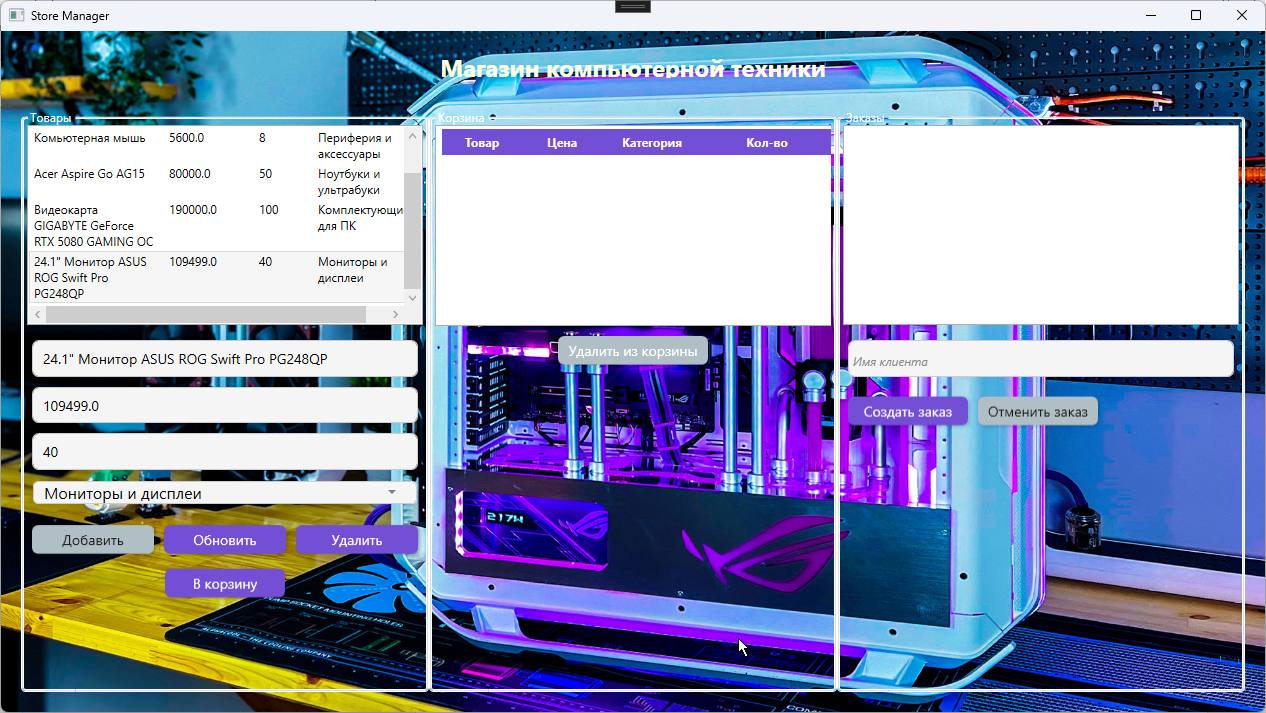
\includegraphics[width=0.8\textwidth]{fig/Рисунок 6.1.png}
	\caption{Главная форма приложения с разделами «Товары», «Корзина» и «Заказы».}
	\label{fig:main_form}
\end{figure}

Пользователь может добавлять новые товары, а также редактировать уже созданные с помощью соответствующих полей и кнопок. Для редактирования товара необходимо выбрать его в списке, нажать на него и его данные будут подставлены в соответствующие поля. После изменения информации необходимо нажать кнопку «Обновить». Для добавления нового товара необходимо ввести данные в соответствующие поля и нажать кнопку «Добавить».

При нажатии кнопки «В корзину» выбранные товары добавляются в блок «Корзина». У пользователя есть возможность управлять количеством товаров, увеличивая или уменьшая его. Ограничение – количество товаров на складе.
Добавление товаров в корзину изображено на рисунке \ref{fig:add_to_cart}.

\begin{figure}[H]
	\centering
	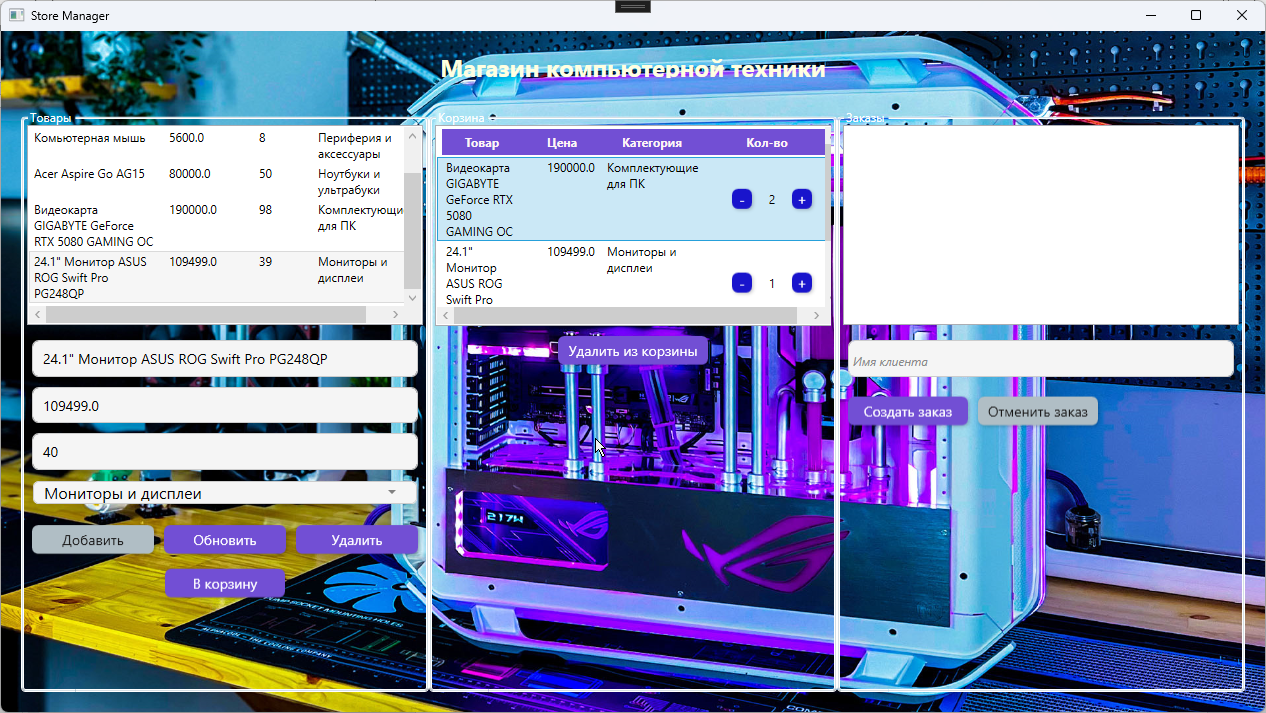
\includegraphics[width=0.8\textwidth]{fig/Рисунок 6.2.png}
	\caption{Добавление товаров в «Корзину».}
	\label{fig:add_to_cart}
\end{figure}

Также у пользователя есть возможность удалить товар из корзины с помощью кнопки «Удалить из корзины» (Рисунок \ref{fig:remove_from_cart}). После удаления товара соответствующее количество товара вернется на склад.

\begin{figure}[H]
	\centering
	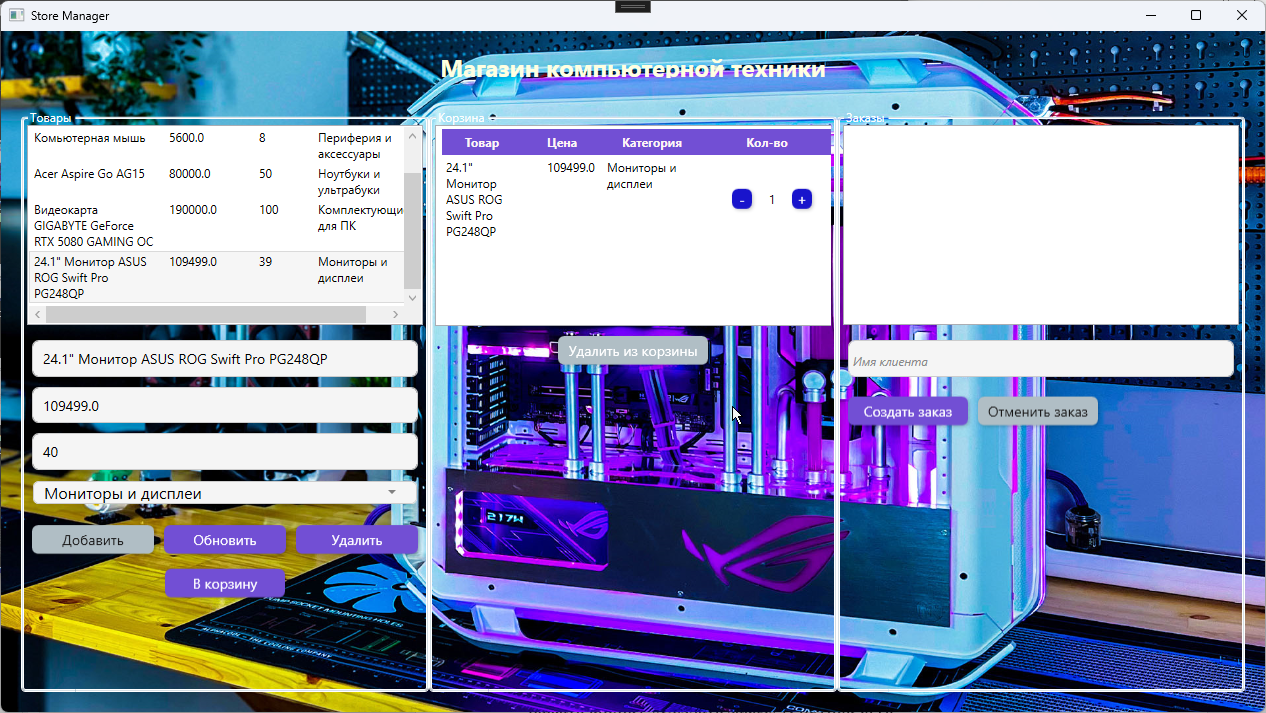
\includegraphics[width=0.8\textwidth]{fig/Рисунок 6.3.png}
	\caption{Удаление выбранного товара.}
	\label{fig:remove_from_cart}
\end{figure}

После выбора необходимых товаров можно добавить новый заказ. Для создания заказа необходимо ввести имя клиента в соответствующее поле и нажать кнопку «Создать заказ» (Рисунок \ref{fig:create_order}).

\begin{figure}[H]
	\centering
	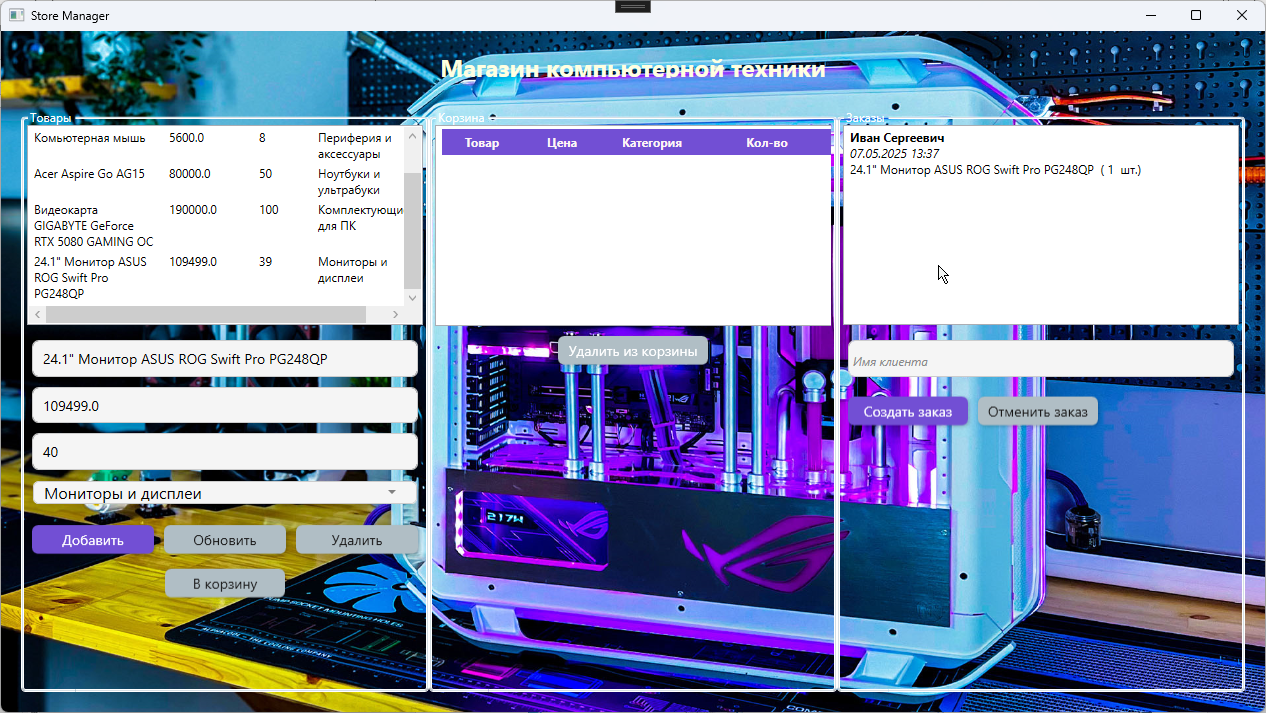
\includegraphics[width=0.8\textwidth]{fig/Рисунок 6.4.png}
	\caption{Пример создания заказа.}
	\label{fig:create_order}
\end{figure}

При попытке добавить новый заказ не добавляя товары в корзину будет выведено соответствующее сообщение (Рисунок \ref{fig:order_error}).

\begin{figure}[H]
	\centering
	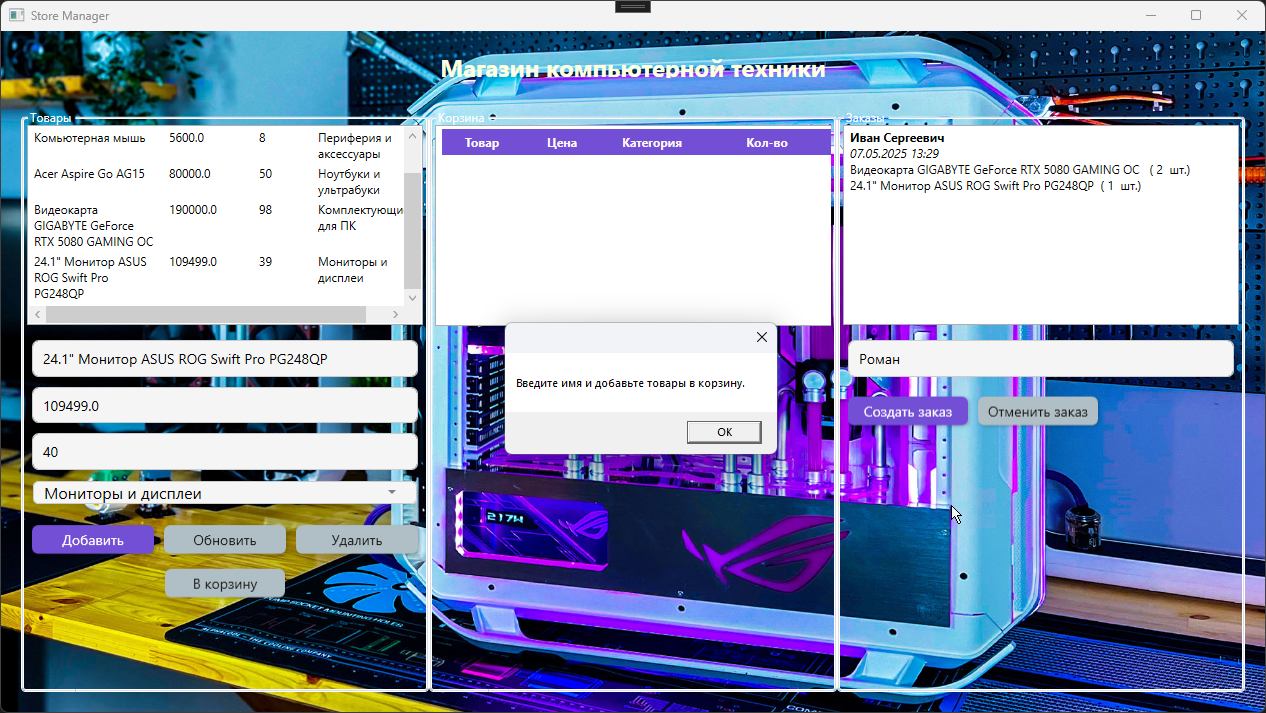
\includegraphics[width=0.8\textwidth]{fig/Рисунок 6.5.png}
	\caption{Ошибка при создании заказа без товаров.}
	\label{fig:order_error}
\end{figure}

Пользователь может отменить заказ нажав на кнопку «Отменить заказ», после этого заказ удаляется из списка заказов.

\section{Контрольные вопросы~\texorpdfstring{\iicon{}}{}}
\begin{enumerate}
	\item \textbf{Что такое MVVM-паттерн и какова его структура в рамках WPF-приложения Store\-Manager?}

	      MVVM (Model-View-ViewModel) — это архитектурный шаблон, применяемый в WPF для разделения представления (XAML), логики отображения (ViewModel) и бизнес-логики (Model). В проекте StoreManager он представлен View (XAML), ViewModel-классами (\texttt{MainViewModel}, \texttt{ProductViewModel}, \texttt{OrderViewModel}) и моделями (\texttt{Product}, \texttt{Order}, \texttt{OrderItem}, \texttt{CartItem}).

	\item \textbf{Как реализована связь между View и ViewModel в WPF-приложении? Приведите пример привязки.}

	      Связь реализована через механизм data binding. Пример: \texttt{Text=''{Binding ProductName}''} привязывает значение поля к свойству во ViewModel. Контекст задаётся через \texttt{Window.DataContext}.

	\item \textbf{Какие классы представляют модель предметной области (Model) в данном проекте и за что они отвечают?}

	      \texttt{Product} — товар, \texttt{Order} — заказ, \texttt{OrderItem} — позиция в заказе, \texttt{CartItem} — товар в корзине. Эти классы хранят бизнес-данные и реализуют интерфейс \texttt{INotifyPropertyChanged}.

	\item \textbf{Какие задачи решает класс \texttt{RelayCommand} и как обеспечивается управление доступностью команд?}

	      Класс \texttt{RelayCommand} реализует интерфейс \texttt{ICommand} и позволяет связать действия UI с методами ViewModel. Доступность определяется функцией \texttt{CanExecute}, обновление — через событие \texttt{CanExecuteChanged}.

	\item \textbf{Как работает механизм уведомления \texttt{INotifyPropertyChanged} в контексте классов \texttt{Product}, \texttt{CartItem} и ViewModel?}

	      При изменении свойства вызывается \texttt{OnPropertyChanged}, которое инициирует событие \texttt{Proper\-tyChanged}. Это позволяет автоматически обновлять связанные элементы UI.

	\item \textbf{Как осуществляется доступ к базе данных с помощью Entity Framework Core в \texttt{StoreDb\-Context}?}

	      Класс \texttt{StoreDbContext} наследуется от \texttt{DbContext} и предоставляет доступ к таблицам через \texttt{DbSet<>}. Настройки соединения и поведения моделей задаются в \texttt{OnConfiguring} и \texttt{OnModel\-Creating}.

	\item \textbf{В чём различие между \texttt{ProductRepository} и \texttt{OrderRepository} по архитектуре и взаимодействию с БД?}

	      \texttt{ProductRepository} работает с одной таблицей \texttt{Product} и выполняет простые SQL-запросы. \texttt{OrderRepository} работает с двумя таблицами (\texttt{Order}, \texttt{OrderItem}) и управляет транзакциями и связями между сущностями.

	\item \textbf{Опишите этапы формирования нового заказа. Какие сущности при этом задействуются?}

	      Пользователь добавляет товары в корзину (\texttt{CartItem}), затем оформляет заказ (\texttt{Order}), в который входят позиции (\texttt{OrderItem}) и клиентские данные. Все объекты сохраняются в базу через \texttt{StoreDbContext} или \texttt{OrderRepository}.

	\item \textbf{Какие команды реализованы в \texttt{MainViewModel}, и как они используются в интерфейсе пользователя?}

	      Команды: \texttt{AddProductCommand}, \texttt{UpdateProductCommand}, \texttt{DeleteProductCommand}, \texttt{AddOrderCommand}, \texttt{DeleteOrderCommand}, \texttt{AddToCartCommand}, \texttt{RemoveFromCartCommand} и др. Каждая команда связана с кнопкой в UI и вызывает соответствующий метод ViewModel.

	\item \textbf{Как реализуется удаление заказа и восстановление остатка товара на складе при этом действии?}

	      При удалении заказа вызывается метод \texttt{DeleteOrder}. Он возвращает количество товаров из заказа обратно в остатки соответствующих \texttt{Product}, после чего заказ удаляется из базы данных.
\end{enumerate}

\end{document}
